Der Versuchsaufbau setzt sich zusammen aus einem Geiger-Müller-Zählrohr, einer Strahlungsquelle, einem Amperemeter, einem Impulszähler und einem Spannungsgenerator (Abb. \ref{fig:aufbau}).
\begin{figure}[h!]
  \centering
  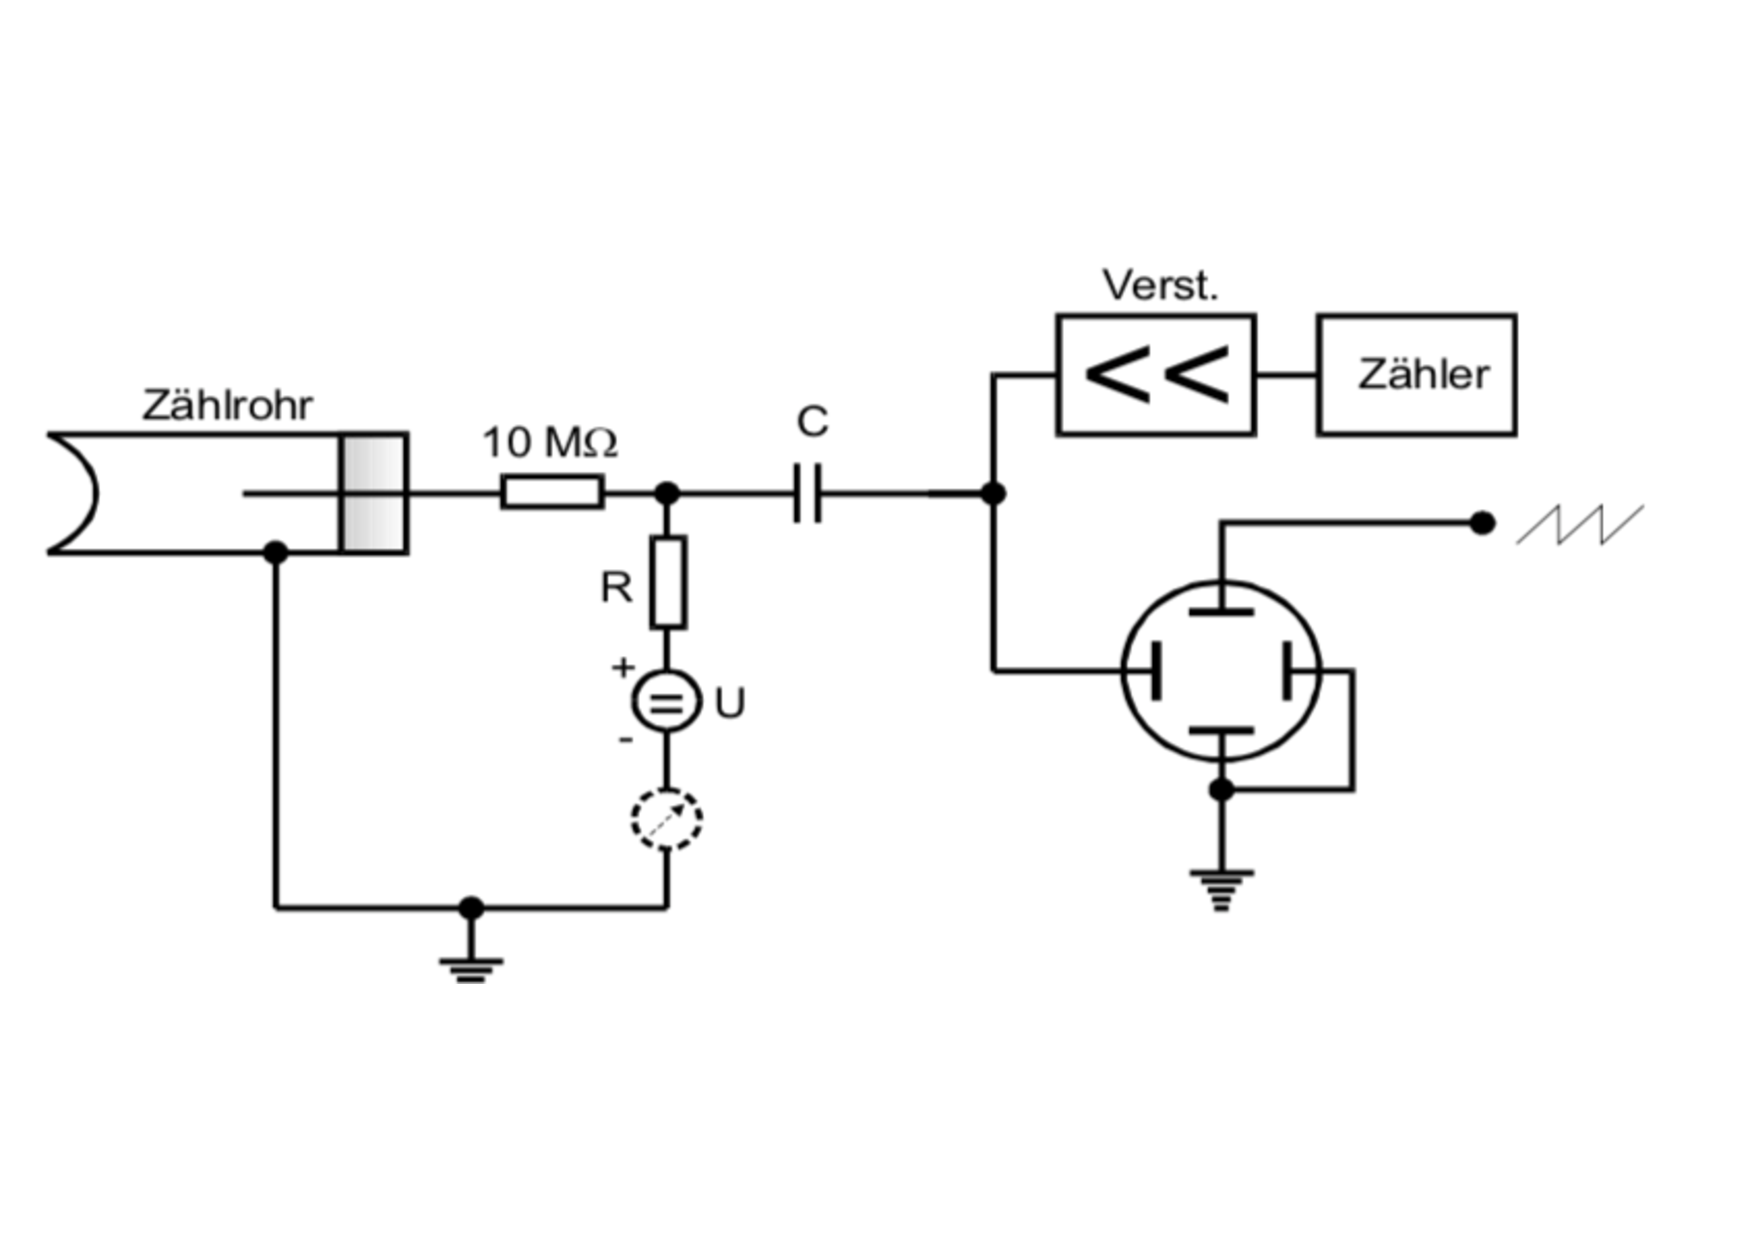
\includegraphics[width=\textwidth]{703aufbau.pdf}
  \caption{Aufbau der Messapparatur \cite{1}}
  \label{fig:aufbau}
\end{figure}
Für die Aufnahme der Zählrohrcharakteristik und für die Messung der Ladungsmenge pro Teilchen werden die Impulse $N$ in einer Minute, der Strom $I$ und die Spannung $U$ notiert.
$U$ wird von $\SI{300}{V}$ bis $\SI{700}{V}$ in $\SI{10}{V}$-Schritten verändert.
Anschließend werden auf dem Oszilloskop die Zeit bis zur Nachentladung, die Totzeit $T_{T}$ und die Erholungszeit $T_{E}$ abgelesen.
Danach wird für die Spannung $U=\SI{560}{V}$ die Zählrate $N$ gemessen.
Zu der ersten Strahlungsquelle wird eine zweite hinzugefügt.
Nun wird für die selbe Spannung die Zählrate $N$ gemessen.
Schließlich wird nur die zweite Strahlungsquelle vermessen.
